% THIS IS SIGPROC-SP.TEX - VERSION 3.1
% WORKS WITH V3.2SP OF ACM_PROC_ARTICLE-SP.CLS
% APRIL 2009
%
% For tracking purposes - this is V3.1SP - APRIL 2009

\documentclass{acm_proc_article-sp}
\usepackage[utf8]{inputenc}
\usepackage[T1]{fontenc}
\usepackage[ngerman]{babel}
\usepackage{amsmath}
\usepackage{graphicx}
\usepackage{amssymb}
\usepackage{fancyhdr}
\usepackage{enumerate}
\usepackage{enumitem}
\usepackage{stmaryrd}

\begin{document}

\title{Documentation zur JEngine}
\numberofauthors{1} 

%
%
\author{
\alignauthor
Jaspar, Jan, Sven, Stephan, Juliane, Jannik\\
       \affaddr{Hasso Plattner Institute}\\
       \affaddr{Prof.-Dr.-Helmert-Str. 2-3}\\
       \affaddr{14482 Potsdam, Germany}\\
       \email{\footnotesize  \{Jaspar,Jan,Sven,Stephan,Juliane,Jannik\}@student.hpi.de}
}
\date{28 December 2014}

\maketitle

%
%
\begin{abstract}
Diese Dokumentation ist entstanden im Rahmen des Bachelorprojekts BP2014W1 am Lehrstuhl für ``Business Process Technology'' betreut durch Prof. Dr. Matthias Weske. Es dient zu Dokumentierung der konzipierten und implementierten JEngine um ein Proof-of-Concept zu ermöglichen und gleichzeitig als Prototype für Anwendungsfälle von Bosch Software Innovations zu fungieren.
\end{abstract}

%
%
\section{Introduction}
Productive Case Management (PCM) beschreibt eine.... \cite{ImplementationFrameworkPCM} (siehe Abbildung \ref{fig:PCMmetaModell}).

%
%
\section{MetaModell}

\begin{figure}
\centering
%\psfig{file=rosette.ps, height=1in, width=1in,}
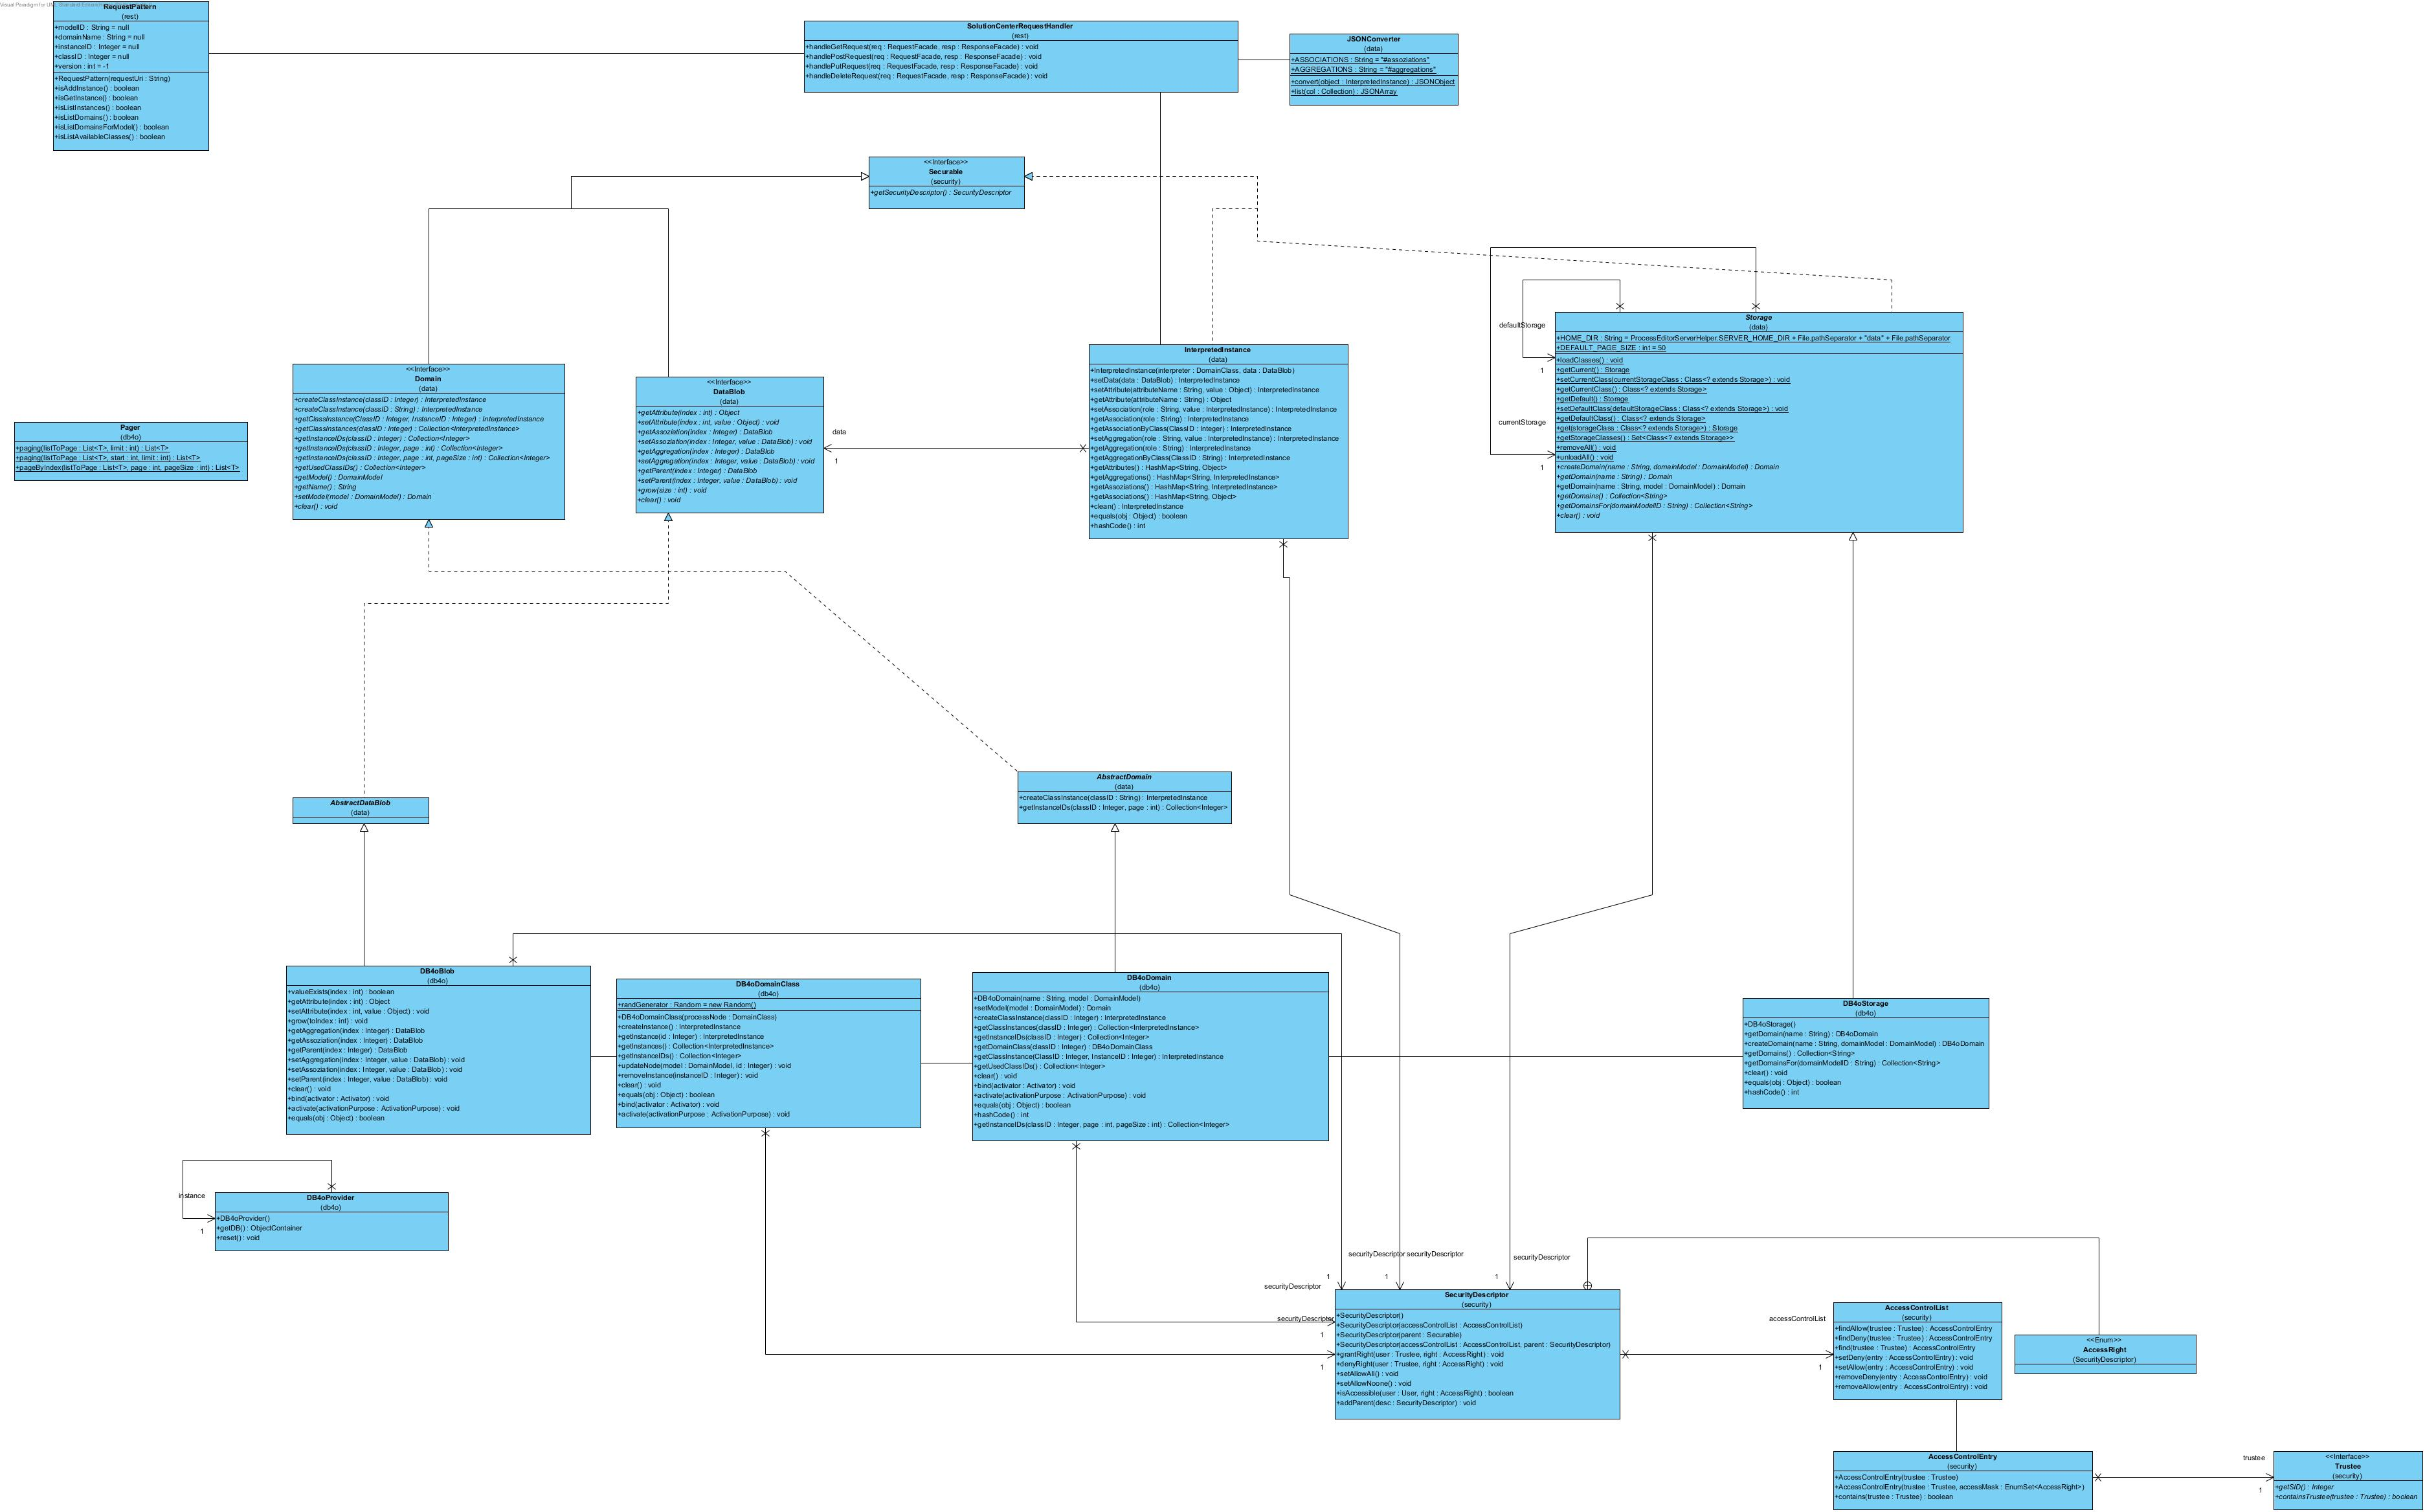
\includegraphics[width=3in]{img/MetaModell_classDiagramm.jpg}
\caption{Meta Modell von PCM.}
\label{fig:PCMmetaModell}
\end{figure}

%
%
\section{JEngine}
Overall JEngine

%
%
\subsection{JCore}
Der JCore umfasst mehrere Hauptkomponenten unserer Engine. Dazu zählt die Auswertung der Datenbank und das Entscheiden von enableden Aktivitäten etc.\\
Dazu zählt zum Beispiel auch die REST-API.

%
%
\subsubsection{REST-API}
Um eine Kommunikation zwischen unseren verschieden Elementen der Engine und des Front-Ends zu ermöglichen, haben wir uns für ein REST-Interface entschieden. Dabei unterstützen wir bisher 2 Methoden: GET und POST.
\begin{enumerate}
%hier beginnt Aufzählung unserer REST Methoden
\item \textbf{@GET:}\\
Die GET-Requests existieren, um den Nutzern der Engine über ein User Interface eine Möglichkeit zu bieten, einzusehen welche Aktivitäten noch zu bearbeiten sind (also offen sind) bzw. welche Aktivitäten zu welcher Scenarioinstanz gehören und ähnliches. \\

Um offene bzw. geschlossene Aktivitäten einer ScenarioInstanz ausgegeben zu bekommen, muss ein GET mit folgender URL ausgeführt werden:\\
\textbf{\textit{http://172.16.64.113:8080/JEngine/Scenario/\\\{ScenarioID\}/\{ScenarioInstanceID\}/\{Status\}}}\\
\textbf{Variablen die benutzt werden:}\\
\textit{ScenarioID:} hier wird die ID des Scenarios erwartet. Dabei handelt es sich um einen Integer-Wert.\\
\textit{ScenarioInstanceID:} hier wird die ID der ScenarioInstanz erwartet. Dabei handelt es sich um einen Integer-Wert.\\
\textit{Status:} Der Status ist vom Typ String und muss ein Element der Menge\textbf{\textit{\{terminated, enabled\}}} sein.\\

\textbf{Dabei können folgende Fehler geworfen werden:}\\
\textit{Error: not a correct scenario instance} Dies bedeutet das eine ScenarioInstanzID angegeben worden ist, die nicht existiert.\\
\textit{Error: status not clear} Dieser Fehler besagt, dass ein Status angegeben wurde, der nicht der Menge \textbf{\textit{\{terminated, enabled\}}} entspricht.\\

\textbf{\textit{http://172.16.64.113:8080/JEngine/Scenario/Show}}\\
\textbf{\textit{http://172.16.64.113:8080/JEngine/Scenario/Instances/\\\{ScenarioInstanceID\}}}\\
throw: Error: not a correct scenario\\
\textbf{\textit{http://172.16.64.113:8080/JEngine/Scenario/DataObjects/\\\{ScenarioID\}/\{ScenarioInstanceID\}}}\\
throw: Error: not a correct scenario instance\\
\textbf{\textit{http://172.16.64.113:8080/JEngine/Scenario/Get/\\ScenarioID/\{ScenarioInstanceID\}}}\\
throw: Error: not a correct scenario instance\\\\

\item \textbf{@POST:}\\


\textbf{http://172.16.64.113:8080/JEngine/Scenario/\\ScenarioID/ScenarioInstanceID/activityID/status/comment}\\
Status = \{terminate, begin\}\\
e.g. \textbf{http://172.16.64.113:8080/JEngine/Scenario/1/47/4/\\terminate/comment}\\
\textbf{http://172.16.64.113:8080/JEngine/Scenario/1/47/4/begin/\\comment}\\
\textbf{http://172.16.64.113:8080/JEngine/Scenario/Start/\\\{ScenarioID\}}\\
throw: -1 (Dann wenn es kein Scenario mit der ID gibt)\\
%
%
\end{enumerate}
\subsubsection{ExecutionService}

%
%
\subsection{JComparser}

%
%
\subsection{JFrontEnd}

%
%
\subsection{JDatabase}

%
%
\section{Processeditor}

%
%
\section{PCM modelling using the Processeditor}\label{pcm-modelling-using-the-processeditor}
This document explains how to use the Processeditor to create PCM
models. A PCM-Process can be described by many PCM fragments and one PCM
scenario.

%
%
\subsection{Preparations}\label{preparations}
Currently you need both, the Processeditor Workbench and the
Processeditor Server to model and Save PCM. You will use the Workbench
for modelling and the Server as a global repository.

%
%
\subsection{PCM Fragments}\label{pcm-fragments}

PCM Fragments are small Business Process models. They can be modelled
using a subset of the BPMN-Notation:

\begin{itemize}
\itemsep1pt\parskip0pt\parsep0pt
\item
  Tasks
\item
  Events ** Blanko Start-Event ** Blanko End-Event
\item
  Gateways ** Parallel Gateway ** Exclusive Gateway
\item
  Data Objects
\item
  Sequence Flow
\item
  Data Flow
\end{itemize}

All this elements are offered by the model type PCM Fragment.

%
%
\subsubsection{Marking a Task as Global}\label{marking-a-task-as-global}
PCM allows to use the same task in more than one fragment. To do so

\begin{enumerate}
\def\labelenumi{\arabic{enumi}.}
\itemsep1pt\parskip0pt\parsep0pt
\item
  model the Task (in one scenario)
\item
  Save the model to the repository
\item
  Right click on the Task and choose \emph{Properties}
\item
  Set the \emph{global flag}
\end{enumerate}

%
%
\subsubsection{Copy and Refer an existing
Task}\label{copy-and-refer-an-existing-task}

\begin{enumerate}
\def\labelenumi{\arabic{enumi}.}
\itemsep1pt\parskip0pt\parsep0pt
\item
  In another Fragment right click on any node
\item
  Choose ``Copy and Refer Task''
\item
  Connect to the server if necessary
\item
  Choose the Model and the Task you want to refer
\item
  Click on Ok
\end{enumerate}

%
%
\subsection{PCM Scenario}\label{pcm-scenario}
A Scenario defines which PCM Fragments are part of one Process. All PCM
Fragments have to be saved on the Server. You can alter the Scenario
only by moving the nodes and adding/removing PCM Fragments.

%
%
\subsubsection{Defining a PCM Scenario}\label{defining-a-pcm-scenario}

\begin{enumerate}
\def\labelenumi{\arabic{enumi}.}
\itemsep1pt\parskip0pt\parsep0pt
\item
  Create a new PCM Scenario Model.
\item
  Right Click on one of the two nodes
\item
  Choose Add Fragments
\item
  Mark all Models you want to add in the left List (CTRL for multi
  select)
\item
  click on add than on ok
\end{enumerate}

Now there should be entries for all the fragments (inside green node)
and for all their data objects (inside white node).

\subsubsection{Removing a Fragment From an
Scenario}\label{removing-a-fragment-from-an-scenario}

\begin{enumerate}
\def\labelenumi{\arabic{enumi}.}
\itemsep1pt\parskip0pt\parsep0pt
\item
  Right Click on one of the two nodes
\item
  Choose \emph{Add Fragments}
\item
  Select all the models you want to remove from the right list
\item
  Click on \emph{Remove} than click \emph{Ok}
\end{enumerate}

\subsubsection{Set a Termination
Condition}\label{set-a-termination-condition}

If a termination condition is full filled the process is terminated.
Currently only one termination condition consisting of one Data Object
in one specific state is possible.

\begin{enumerate}
\def\labelenumi{\arabic{enumi}.}
\itemsep1pt\parskip0pt\parsep0pt
\item
  Open your Scenario
\item
  Right Click on the canvas (not the Nodes)
\item
  Choose \emph{Properties}
\item
  Fill out the \emph{Termination Data Object} and \emph{Termination
  State} fields
\end{enumerate}

\subsubsection{Copy and Alter a Complete
Fragment}\label{copy-and-alter-a-complete-fragment}

You can create a variation of an existing PCM Fragment using the Plug-in
\emph{Create Variant}.

\begin{enumerate}
\def\labelenumi{\arabic{enumi}.}
\itemsep1pt\parskip0pt\parsep0pt
\item
  First click on \emph{Plug-Ins}
\item
  Choose \emph{Create Variant}
\item
  Choose your Fragment and click on \emph{Ok}
\end{enumerate}


%
%
\subsection{Processeditor Server}


%
%
\subsection{Processeditor Client}


%
%
\bibliographystyle{abbrv}
%\bibliographystyle{unsrt}
\bibliography{JEngine-docu} 

%
%
\end{document}
